
\subsection{Primer diseño}

A partir de una selección del video proporcionada por el usuario se obtienen las mejores features del objeto deseado, utilizando el algoritmo de Shi-Tomasi. Luego, mediante el de Lucas-Kanade de Optical Flow se obtiene la evolución de dichas features en el tiempo. A este cúmulo de puntos se le calcula el centro de masas $\mu$ y el centro de inercia $\sigma$. Se rechazan los puntos de este cúmulo que se encuentren a una distancia mayor a $k_{\sigma}\sigma$ respecto al centro de masas, para luego calcular nuevamente dicho centro, el cual es el que se introduce en el filtro de Kalman como medición de la posición.

La dimensión del vector de estados del filtro de Kalman es de cuatro, poseyendo la posición y la velocidad tanto horizontal como vertical. La dimensión del vector de observación es de dos, dado que solamente se mide la posición horizontal y vertical del centro de masas. La matriz $A$ queda definida por las ecuaciones que caracterizan el movimiento del objeto a seguir que, por simplicidad, se consideraron las ecuaciones cinemáticas de MRU, quedando entonces
\begin{equation}
\begin{pmatrix} x_{k-1} + dt\cdot v_{x_{k-1}} \\y_{k-1} + dt\cdot v_{y_{k-1}} \\ v_{x_{k-1}}  \\ v_{y_{k-1}} \end{pmatrix} =\begin{pmatrix}
1 & 0 & dt  & 0\\
0 & 1  & 0 & dt\\
0 & 0  & 1  & 0\\
0 & 0  & 0  & 1 
\end{pmatrix} \cdot \begin{pmatrix} x_{k-1}\\y_{k-1} \\ v_{x_{k-1}}  \\ v_{y_{k-1}} \end{pmatrix}
\end{equation}
Siendo, 
\begin{equation}
A = 
\begin{pmatrix}
1 & 0 & dt  & 0\\
0 & 1  & 0 & dt\\
0 & 0  & 1  & 0\\
0 & 0  & 0  & 1 
\end{pmatrix}
\end{equation}

Luego, se tiene que la matriz de observación o de transición de medición queda definida por la transformación del espacio de observación al espacio real del vector de estados del filtro. Como los observables a medir forman parte del espacio real del vector de estados y son solo las posiciones, la matriz queda definida de manera simple
\begin{equation}
\begin{pmatrix} z_{x_{k}} \\ z_{y_{k}} \end{pmatrix}=\begin{pmatrix}
1 & 0 & 0  & 0\\
0 & 1  & 0 & 0  \end{pmatrix} \cdot  \begin{pmatrix} x_k \\ y_k \\ v_{x_{k}} \\ v_{y_{k}}
\end{pmatrix}
\end{equation}
Siendo,
\begin{equation}
H = 
\begin{pmatrix}
1 & 0 & 0  & 0\\
0 & 1  & 0 & 0 
\end{pmatrix}
\end{equation}

Las matrices de covarianza del proceso $Q$ y de medición $R$ son cuadradas por definición, de dimensión cuatro y dos respectivamente. Además, son la forma $\mathbb{I}\cdot \xi$ dado que se asume independencia de las variables aleatorias, quedando

\begin{equation}
Q = 
\begin{pmatrix}
\xi_Q & 0 & 0  & 0\\
0 & \xi_Q  & 0 & 0\\
0 & 0  & \xi_Q  & 0\\
0 & 0  & 0  & \xi_Q 
\end{pmatrix}
\end{equation}

\begin{equation}
R = 
\begin{pmatrix}
\xi_R & 0 \\
0 & \xi_R 
\end{pmatrix}
\end{equation}
Siendo $\xi_Q$ y $\xi_R$ las varianzas del proceso y de medición respectivamente.

Finalmente, $\hat{x}_{k|k}$ y $P_{k|k}$ toman la forma

\begin{equation}
\hat{x}_{k|k} = 
\begin{pmatrix}
\hat{x}\\
\hat{y}\\
\hat{v_x}\\
\hat{v_y}
\end{pmatrix}
\end{equation}

\begin{equation}
P_{k|k} = 
\begin{pmatrix}
\gamma_{x} & 0 & 0  & 0\\
0 & \gamma_{y}  & 0 & 0\\
0 & 0  & \gamma_{v_x}  & 0\\
0 & 0  & 0  & \gamma_{v_y} 
\end{pmatrix}
\end{equation}
Siendo $\gamma_{i}$ la varianza de cada variable de estado. Cabe notar que el modelo utilizado asume independencia entre las variables aleatorias por simplicidad.

Este algoritmo explicado, cuenta con grandes problemas. Dados dos objetos $A$ y $B$, donde $A$ es el objeto a seguir:

\begin{itemize}
\item Como el algoritmo de Shi-Tomasi tiende a colocar features en bordes bien definidos, y estos suelen ser los bordes externos de un objeto, si el objeto a seguir $A$ pasa por delante de un objeto $B$ con bordes bien definidos, las features del algoritmo de Optical Flow tienden a adosarse a los bordes del objeto $B$ por más que este esté quieto.
\item Si el objeto $A$ pasase por detrás del objeto $B$ inmóvil, todas las features sobre el objeto a seguir quedan adosadas al objeto $B$. Esto plantea un problema mucho más grande que el anterior, dado que no se puede utilizar la estimación del filtro de Kalman de manera confiable, debido a que cuando los features se queden quietos adosados en $B$, se sigue midiendo de todas formas y se sigue entregando esas mediciones al filtro de Kalman, por lo que la estimación de este se adosa también al objeto $B$.
\item Profundizando en el item anterior, existe una ambigüedad entre que $A$ pase de un movimiento MRU a que se quede completamente quieto y que $A$ pase por detrás de $B$, dado que en ambas situaciones las features quedan quietas en el lugar donde $A$ se haya quedado quieto o el lugar de la intersección entre $A$ y $B$
\end{itemize}




























\subsection{Segundo diseño}

\subsubsection{Enmascaramiento Basado en HSV}

La mejora propuesta para sortear estos problemas consiste en agregar un filtro de color, para diferenciar a $A$ y a $B$ por su color. La implementación de este filtro de color comienza en el momento en el que el usuario selecciona el área a seguir. Se calcula la mediana del color de la zona elegida, y ese color es transformado de formato RGB a formato HSV, o Hue-Saturation-Value, dado que es más sencillo definir una máscara de este modo. Dado $x$ e $y$ las coordenadas de los píxeles de la imagen, $\vec{R_k}$, $\vec{G_k}$ y $\vec{B_k}$ los vectores de píxeles de la selección, $mediana(\vec{R_k}, \vec{G_k}, \vec{B_k}) = (m_R, m_G, m_B)$ el vector que define la mediana del color de la selección, $\mathbb{HSV}$ el operador de transformación del espacio de coordenadas RGB a HSV, y $\mathbb{HSV}(m_R, m_G, m_B) = (m_H, m_S, m_V)$ el vector de la mediana del color de la selección en el espacio HSV, queda entonces definida la máscara de color como

\begin{equation}
f(x, y) = (f_h(x, y), f_s(x, y), f_v(x, y))
\end{equation}

\begin{equation}
f_{u}(x,y) = \left\{
\begin{array}{ll}


      1 & -\Lambda_u < u_{x, y} - m_u < \Lambda_u \\
      
      
      
      0 & \text{sino} \\
      
      
\end{array} 
\right.
\end{equation}

donde $\Lambda$ es el límite para cada propiedad $u$, siendo estas Hue, Saturation o Value. Una vez obtenida la máscara $f(x, y)$ se realiza la operación AND entre la máscara y la imagen original, logrando obtener una intensidad nula en los píxeles de la imagen que no posean un color cercano a la mediana calculada como se puede ver en las Figuras (\ref{fig:col1}) y (\ref{fig:col2}).

\begin{figure}[H]
\centering
	\begin{subfigure}{.4\textwidth}
		\centering
		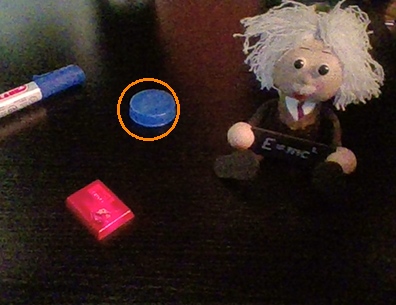
\includegraphics[width=\textwidth]{Imagenes/color1.png}
		\caption{Video antes de aplicar la máscara siguiendo al objeto azul.}
		\label{fig:col1}
	\end{subfigure}
	\begin{subfigure}{.4\textwidth}
		\centering
		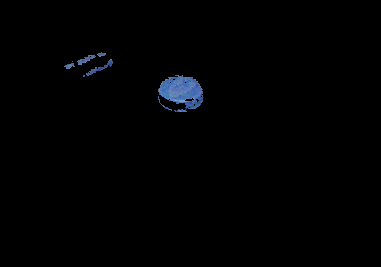
\includegraphics[width=\textwidth]{Imagenes/color2.png}
		\caption{Video después de aplicar la máscara. Es con esta imagen que opera el algoritmo y no con la normal.}
		\label{fig:col2}
	\end{subfigure}
	\caption{Comparación entre video normal y luego de aplicar la máscara.}
	\label{fig:color_comp}
\end{figure}

Este filtrado de color no solo posee una gran sinergia con el método de obtención de features de Shi-Tomasi, dado que este frame tiene bordes de mucha mejor calidad, sino que también posee una gran sinergia con el método de Optical Flow, debido a que como se ven menos bordes en la imagen modificada, aumenta notablemente la probabilidad de que los features queden contenidos todos dentro, o sobre los bordes del objeto a seguir.

Volviendo al caso de los objetos $A$ y $B$:

\begin{itemize}
\item Si $A$ y $B$ son de colores distintos, con el filtro de color, el algoritmo nunca detecta que existe un objeto $B$ por lo que seguirlo es imposible. Por consecuencia, se sigue únicamente a $A$ y no se tiene el problema de $A$ pasando por frente de $B$.
\item Si $A$ y $B$ son de colores distintos, y $A$, el objeto a seguir, pasa por detrás de $B$, ahora no se adosan las features al objeto $B$, sino que el algoritmo ve que el área de $A$ se achica a medida que este queda oculto por $B$. Como los features no tienen bordes para seguir, estos desaparecen, por lo que se deja de entregar mediciones al filtro de Kalman y este estima correctamente la posición de $A$ mientras que este no haya sufrido aceleración alguna mientras estaba oculto. 
\end{itemize}

\begin{figure}[H]
\centering
	\begin{subfigure}{.4\textwidth}
		\centering
		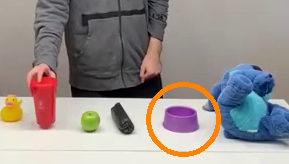
\includegraphics[width=\textwidth]{Imagenes/Optical1.png}
		\caption{Ventana con el funcionamiento normal del seguidor, el cual utiliza un círculo naranja para detallar donde se encuentra el objeto a seguir.}
		\label{fig:optical1}
	\end{subfigure}
	\begin{subfigure}{.4\textwidth}
		\centering
		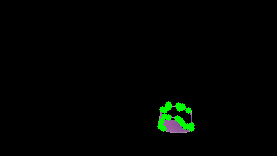
\includegraphics[width=\textwidth]{Imagenes/Optical2.png}
		\caption{Ventana la cual solo aparece al seleccionar el modo debug. Aquí se muestra si el filtro de color se encuentra activado, el video luego de pasar por la máscara de color, las features del objeto como puntos verdes y la zona de búsqueda si se diese el caso de tracking failure.}
		\label{fig:optical2}
	\end{subfigure}
	\caption{Resultado de la selección de un elemento.}
	\label{fig:optical12}
\end{figure}

\subsubsection{Búsqueda del Objeto Perdido}

Sin embargo, el filtro de Kalman no puede estimar la posición del objeto indefinidamente. Es por esto que cuando el objeto se pierde, es decir, no se logran detectar más features, se entra en otra fase del programa. En esta fase, se realiza una búsqueda del objeto en cada frame del video a partir de la estimación del filtro de Kalman y el tamaño original del área seleccionada. La altura y el ancho del área de búsqueda se incrementa por un factor constante por cada frame en la que la búsqueda falle. Esta búsqueda se basa en aplicar el algoritmo de Shi-Tomasi sobre el área mencionada.

\subsubsection{Corrección Periódica de los Puntos Característicos}

Finalmente, para reforzar el algoritmo de seguimiento, se implemento además una recalculación periódica de las features con el método de Shi-Tomasi. Se parte de la media del cúmulo de features, removiendo los outliers, volviendo a calcular nuevamente la media y utilizar esta posición para aplicar el algoritmo de Shi-Tomasi, de la misma manera que se realiza sobre la primera selección proporcionada por el usuario. Todo esto permite subsanar varios de los problemas planteados anteriormente, sin embargo, existen aún otros problemas.

\subsubsection{Escenarios de fallas}
Algunos casos donde puede fallar hasta ahora el Tracker son:
\begin{itemize}
\item El cambio de trayectoria de un objeto una vez que desaparece, provocando una falla en la predicción.
\item Interacción entre el objeto trackeado y un objeto de características similares, causando un error de detección
\item Cambios bruscos de iluminación o en color del objeto.
\end{itemize}































\subsection{Último diseño}

En la última iteración del proceso de diseño se sacrificó bajo costo computacional por una mayor robustez en el algoritmo, reduciendo significativamente las probabilidades de:
\begin{itemize}
\item Error tipo I: no se encuentra el objeto a seguir por más que sea visible.
\item Error tipo II: se detecta un objeto por más que el objeto a seguir no se encuentre en pantalla.
\item Error tipo III: se detecta a otro objeto por más que el objeto a seguir este visible.
\end{itemize}
mediante el uso de \textit{Matched Filters}. Además, se logró obtener una gran robustez frente a cambios en la iluminación utilizando un algoritmo alternativo de enmascaramiento basado en la distribución de hue del objeto a seguir. Por último, se desarrolló una interfaz gráfica donde se puede cargar un video o bien utilizar una cámara en tiempo real, seguir varios objetos a la vez, modificar cualquier parámetro de cualquiera de los algoritmos utilizados en tiempo real e incluso se desarolló un método de optimización automático de los parámetros del algoritmo de enmascaramiento. En la Figura (\ref{gui}) se puede observar una captura de la interfaz gráfica desarrollada y en la Figura (\ref{fig:Flowchart}) se puede observar el diagrama de flujo entero del algoritmo de seguimiento desarrollado. La Figura (\ref{fig:class}) aporta una visión de cómo se organiza el programa mencionado.


\begin{figure*}
	\centering
	\includegraphics[width=0.9\textwidth]{../flowchart.jpg}
	\caption{Flow-chart del algoritmo.}
	\label{fig:Flowchart}
\end{figure*}

\begin{figure*}
	\centering
	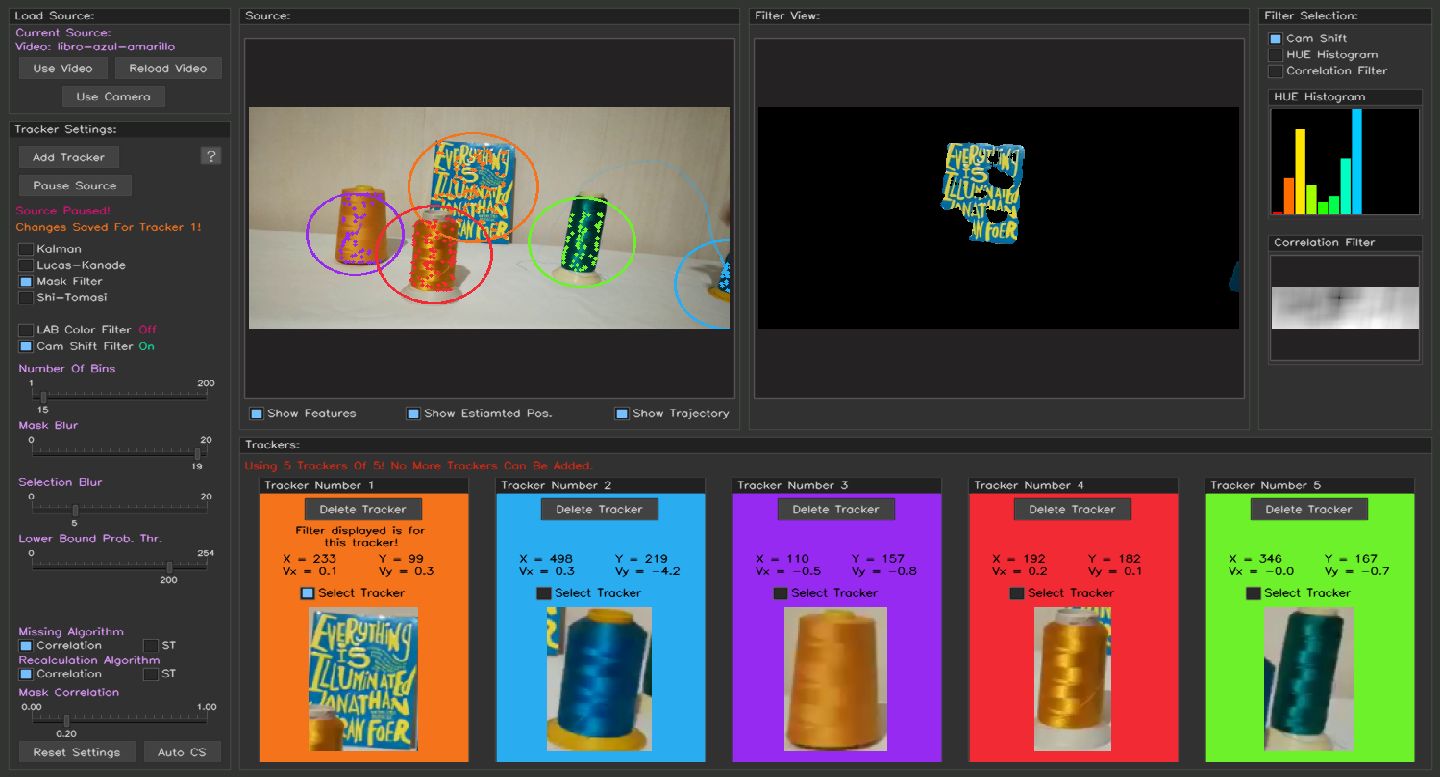
\includegraphics[width=0.9\textwidth]{Imagenes/gui.png}
	\caption{Captura de pantalla de la interfaz gráfica desarrollada.}
	\label{gui}
\end{figure*}

\begin{figure*}
\centering
	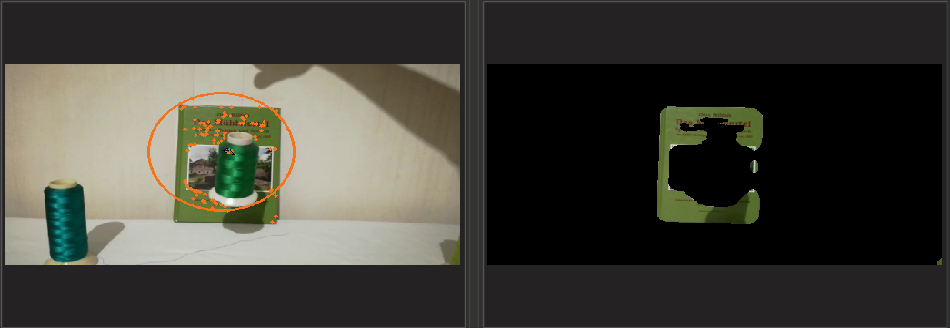
\includegraphics[width=0.8\textwidth]{Imagenes/camshift_mask1.png}
	\caption{Primer ejemplo del algoritmo de enmascaramiento basado en histogramas de hue. En este ejemplo se puede notar la eficiencia conseguida en la máscara, debido a que por más que se encuentren varios objetos en escena de un color muy similar al objeto de interés, estos son exluídos por la máscara. Además, y de mayor importancia, se puede notar como el algoritmo de enmascaramiento no excluye la zona del libro bajo sombra. Esto muestra la gran robustez frente a cambios en la iluminación del algoritmo.}
	\label{fig:c_mask1}
\end{figure*}

\begin{figure}[H]
	\centering
	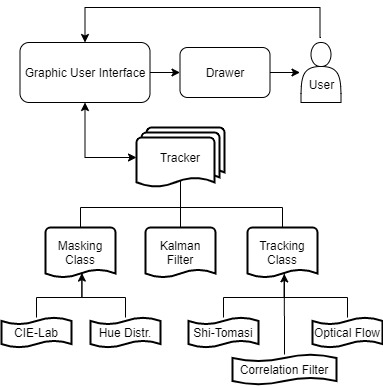
\includegraphics[width=0.45\textwidth]{Imagenes/Classes.jpg}
	\caption{Diagrama de Clases del programa utilizado para presentar la funcionalidad del algoritmo desarollado.}
	\label{fig:class}
\end{figure}




















\subsubsection{Enmascaramiento Basado en CIE-Lab}

El diseño anterior poseía un algoritmo de enmascaramiento basado en el espacio de color HSV. Si bien este funcionaba correctamente, este espacio de color fue reemplazado por CIE-Lab debido a que este posee un solo parámetro que caracteriza la iluminación de un objeto, es decir, con un valor nulo de L se obtiene el negro, mientras que con un valor máximo de L se obtiene blanco, pasando entre medio de esos dos valores por el color representado por a y b. En el espacio HSV, si se utiliza el máximo valor de la componente value, no necesariamente se obtiene blanco, sino que depende del valor de saturación elegido, mientras que si value es nulo, siempre se obtiene negro. Poseer un solo parámetro que correctamente caracterice la iluminación de un objeto brinda una mejor optimización de los valores de semiamplitudes L-a-b utilizados en el enmascaramiento. 

La generación de la máscara se realiza de la misma forma que en el diseño anterior, con el único agregado de un suavizamiento de la máscara computada previo a la utilización de esta para el filtrado de la imagen. Esto se utiliza debido a que generalmente los bordes de un objeto poseen mayor o menor iluminación dependiendo de dónde este la fuente de luz más cercana. Estas diferencias en la iluminación pueden ocasionar que un objeto de similar color al de interés sea vez correctamente excluído de la imagen a excepción de sus bordes, lo cual genera problemas al pasar por delante o por detrás del objeto a seguir por causas detalladas anteriormente.

\begin{figure}[H]
	\centering
	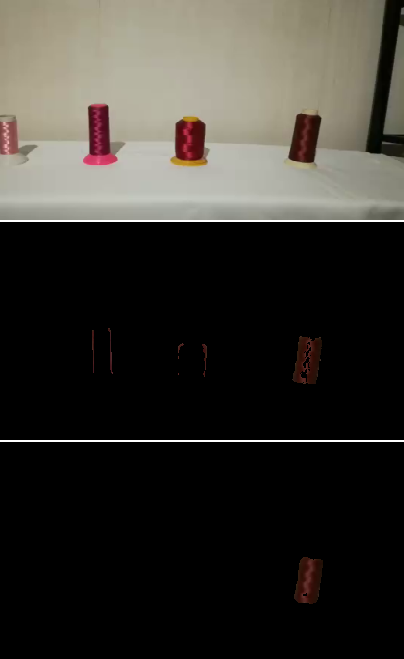
\includegraphics[width=0.45\textwidth]{Imagenes/medianblur.png}
	\caption{Ejemplo del uso del suavizado de la máscara de color. La segunda foto es la máscara previo al suavizado y la tercer foto es posterior al suavizado.}
	\label{fig:medianblur}
\end{figure}

Sin embargo, si bien la utilización del espacio de color CIE-Lab subsanó varios problemas, el enmascaramiento de la imagen tomando en cuenta solamente uno de los varios colores del objeto a seguir falla cuando se encuentra en pantalla un objeto del mismo color que el utilizado para la máscara. Para lidiar con este problema, se decidió desarrollar un método de enmascaramiento que tenga en cuenta todos los colores del objeto a seguir.





















\subsubsection{Enmascaramiento Basado en Histogramas de Hue}
Para este método de enmascaramiento, el espacio de color HSV fue utilizado debido a que un solo parámetro es el encargado de denotar el color, lo cual genera que la distribución de color de un objeto sea una variable aleatoria unidimensional y no bidimensional como lo sería en el espacio de color CIE-Lab. Aclarado esto, los objetos pueden adquirir perfiles de color complejos, sus colores pueden estar distribuidos entorno a un solo valor de hue dominante, o pueden tener más de uno en su composición, obteniendo distribuciones unimodales o multimodales, respectivamente. 
\begin{figure}[H]
	\centering
	\begin{subfigure}{.4\textwidth}
		\centering
		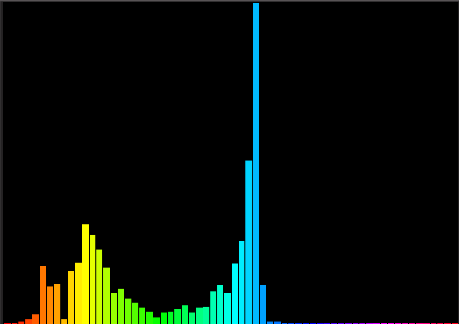
\includegraphics[width=0.8\textwidth]{Imagenes/camshift_hist_bimodal.PNG}
		\caption{Distribución de color bimodal.}
		\label{fig:bimodal}
	\end{subfigure}
	
	\begin{subfigure}{.4\textwidth}
		\centering
		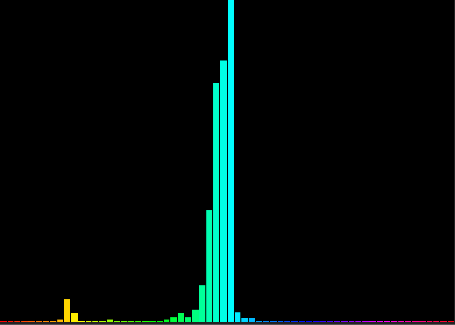
\includegraphics[width=0.8\textwidth]{Imagenes/camshift_hist_unimodal.PNG}
		\caption{Distribución de color unimodal.}
		\label{fig:unimodal}
	\end{subfigure}

\end{figure}
Para obtener una máscara que podamos utilizar debemos establecer un límite para así dejar pasar solamente aquellos pixeles cuyo hue tenga una alta probabilidad de pertenecer al objeto seleccionado. 

\begin{figure}[H]
	\centering
	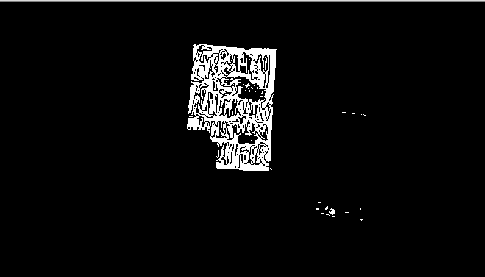
\includegraphics[width=0.32\textwidth]{Imagenes/mascara_bimodal.PNG}
	\caption{Máscara obtenida luego de quedarnos con los pixeles más probables.}
	\label{fig:noisy_lpf}
\end{figure}
Debemos notar en la Figura (\ref{fig:noisy_lpf}) que se pueden observar claramente las letras y el fondo de la tapa del libro. Como se puede apreciar, el histograma del ejemplo presenta una distribución bimodal la cual ha sido exitosamente capturada por el método de filtrado.

\begin{figure}[H]
	\centering
	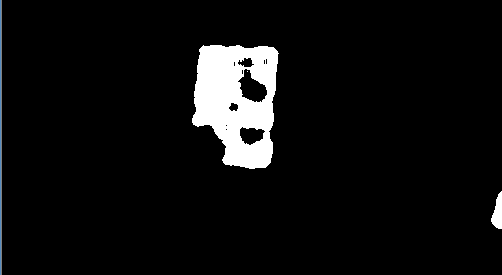
\includegraphics[width=0.32\textwidth]{Imagenes/mascara_bimodal_lpf.PNG}
	\caption{Aplicamos el equivalente a un filtro pasabajos para disminuir el ruido.}
	\label{fig:lpf_hist}
\end{figure}

Sin embargo, la Figura (\ref{fig:noisy_lpf}) presenta ciertos pixeles que pueden interferir con las features calculadas mediante Shi-Tomasi. Es por eso que utilizamos la operación de suavizado para eliminar el ruido. Esto trae acarreado otro beneficio, el interior de la mascara se vuelve más uniforme y permisivo para los pixeles que pertenecen al interior del objeto.
\begin{figure}[H]
	\centering
	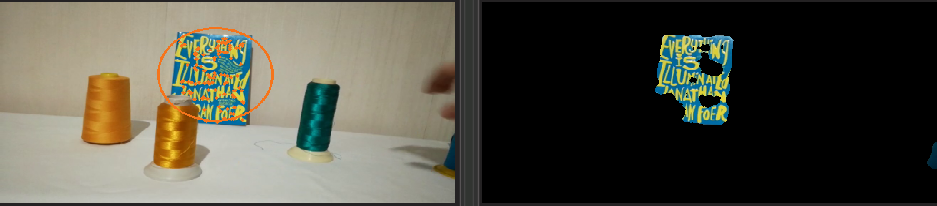
\includegraphics[width=0.5\textwidth]{Imagenes/camshift_mask3.png}
	\caption{Comaparación antes y después del filtrado.}
\end{figure}
 

\begin{figure}[H]
\centering
	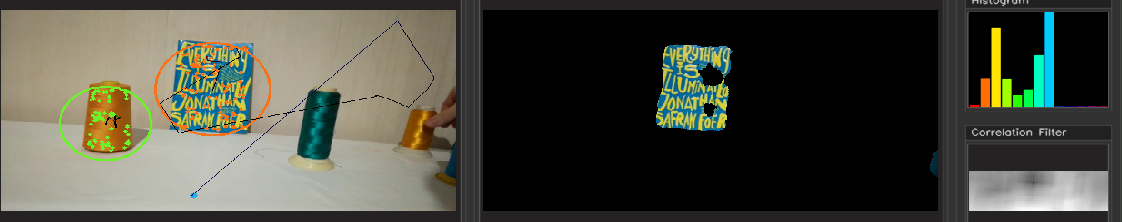
\includegraphics[width=0.45\textwidth]{Imagenes/camshift_mask2.png}
	\caption{Segundo ejemplo del algoritmo de enmascaramiento basado en camshift. Se observa como el enmascaramiento se realiza a partir de la distribución de colores y no de los colores por separado, dado que por más que los carretes de hilo azules y amarillos posean colores dentro de la selección original (el libro), estos son excluídos por el algoritmo de enmascaramiento. Se editó a posteriori el histograma de colores de la selección sobre la imagen ya filtrada.}
	\label{fig:c_mask2}
\end{figure}

























%\subsubsection{Algoritmo de Optimización de los Parámetros del Algoritmo de Enmascaramiento}
%le cambie el nombre a la seccion por este porque seguramente pueda hacer andar optimize.shgo de scipy con el filtro de LAB que tiene los parametros rikis continuos



























\subsubsection{Algoritmo correlación}
Para el algoritmo de correlación no solo se utiliza el filtro explicado en la Sección \ref{sec:corr}, sino que ademas se trata tanto al frame como al kernel, aplicando una transformación al espacio HSV. La trasformación de RGB a HSV posee un requerimiento computacional significativamente menor a la transformación de RGB a CIE-Lab y por eso se utilizó nuevamente el espacio HSV, dado que este filtrado sería complementario al método de la correlación y no lo más importante en el algoritmo. El filtrado se realizó bajo las siguientes especificaciones: 
            
\begin{align}
MSK = H \  \epsilon \ (0,180 ) \ \ S \  \epsilon \ (50,255) \ \ V \ \epsilon \ (32,255)
\end{align}
Este filtrado del kernel logra eliminar aquellos pixeles de muy baja saturación (grises) y de muy bajo valor (negros), lo cual se comprobó experimentalmente que aumenta considerablemente la precisión en el algoritmo.
Luego, se utiliza el filtro de correlación y se obtiene el punto donde esta es mayor. Se toma una sección alrededor de este punto proporcional a la selección inicial y se compara con el frame original. Si no comparten las características de color que son calculadas por el enmascaramiento de color o distribución de color, este punto de correlación es desechado. Esto se logra aplicando una máscara en la sección del frame de mayor correlación, realizando sobre este nuevamente el cálculo de máxima correlación. Este proceso se realiza unas pocas veces con el propósito de no comprometer la velocidad de procesamiento entre frames. En caso de no encontrar al objeto se considera que hubo un error de trackeo (oclusión del objeto).\\

\begin{figure}[H]
\centering

		\begin{subfigure}{.5\textwidth}
		\centering
		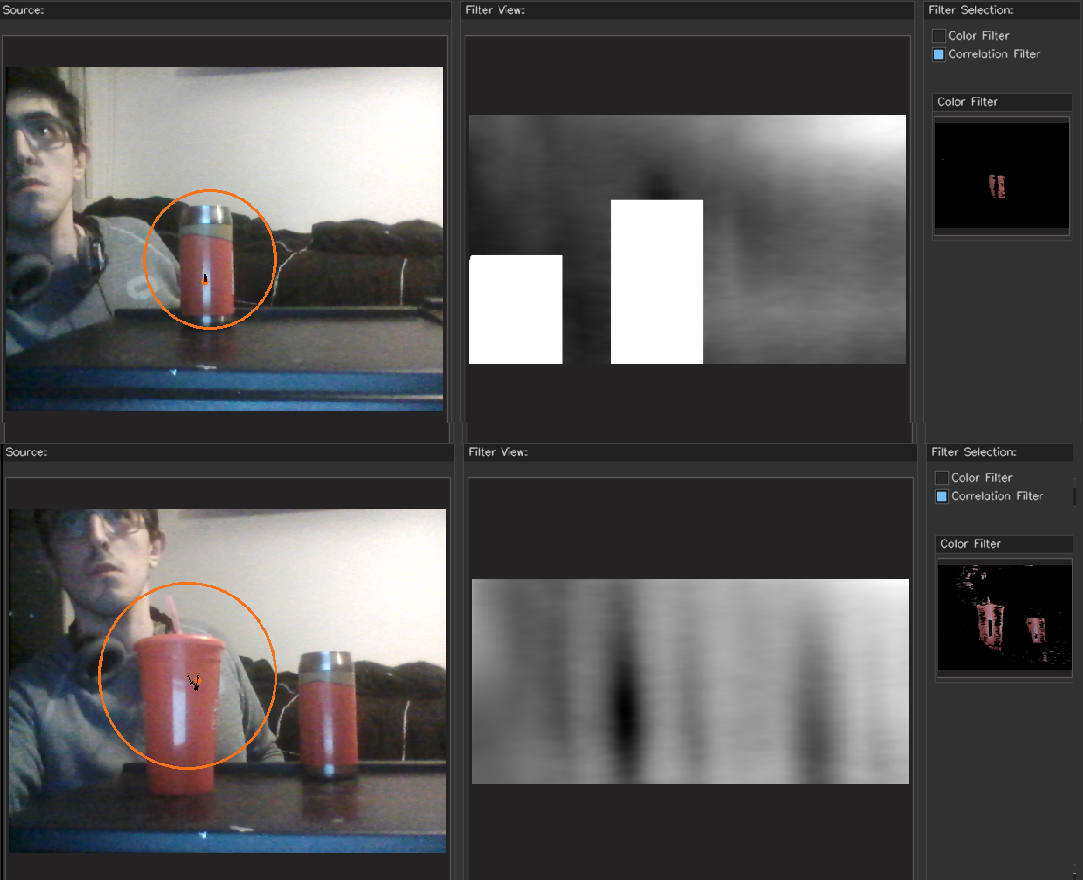
\includegraphics[width=0.75\textwidth]{Imagenes/corrmask.png}
		\caption{Correlación con máscara ante oclusión del objeto}
		\label{fig:sqdiff2}
	\end{subfigure}
	\begin{subfigure}{.1\textwidth}
		\centering
		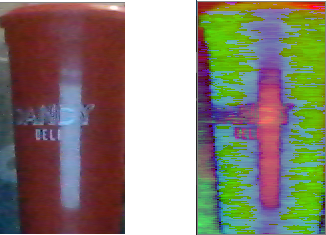
\includegraphics[width=1.5\textwidth]{Imagenes/kernelhsv.png}
		\caption{Kernel}
		\label{fig:kernel2}
	\end{subfigure}
	\caption{Aplicación del algoritmo de correlación con máscara.}
	\label{fig:corrtest2}
\end{figure}

Este algoritmo es utilizado en dos escenarios. En el primero se utiliza para la búsqueda de un objeto perdido. En caso de oclusión se utiliza el algoritmo para encontrar nuevamente el objeto, siendo efectivo siempre que no haya objetos que compartan tanto forma y color con el de interés. Por otro lado, en caso de que así sea y el objeto de interés se encuentre oculto, es posible que el algoritmo devuelva un falso positivo, siendo conviene utilizar el alternativo de Shi-Tomasi y medias móviles, dado que el tener información de la posición previa para el tracking resulta fundamental para poder distinguir entre estos.

El otro escenario es utilizar la correlación para el recálculo periódico de features, esto es beneficioso cuando se da la interacción de dos objetos $A$ y $B$ siendo $A$ el de interés y $B$ uno similar. Si $B$ pasa por delante de $A$ quitandole las features, el cálculo periódico por correlación puede detectar que se está siguiendo a $B$ y no a $A$, por lo que corrige este error. Una situación similar a esta no puede ser resuelta por el algoritmo de Shi-Tomasi con medias móviles.



































\subsubsection{Optimización del Código}
Se realizó una optimización del código, quitando redundancias y utilizando únicamente librerías que son corridas en C++ con la finalidad de que el procesamiento en tiempo real sea eficiente. Se optó por un enfoque OOP, esto permitió escalar el proyecto y obtener una mayor modularidad. \\
Además se diseñó una GUI con la capacidad de trackeo multi-objeto, personalización de algoritmos, contando con la opción de variar algoritmos tanto de búsqueda como de recálculo entre medias móviles y correlación, al igual que filtrado por color o camshift. Existen la opción de cambiar las especificaciones de los filtros en tiempo real para obtener el filtro óptimo o que un algoritmo de optimización las calcule automaticamente. También se permiten diversas pantallas de debug, es decir, observar los ditintos filtros a la vez, al igual que una estimación de la posición y velocidad del objeto. Finalmente cuenta con la capacidad de utilizar tanto un video en tiempo real como un video pre-existente.





% Finalmente se presenta un diagrama en bloques del programa, donde se puede apreciar como interaccionan todos %los algoritmos trabajando en armonía.
%\begin{figure}[H]
%\centering
%	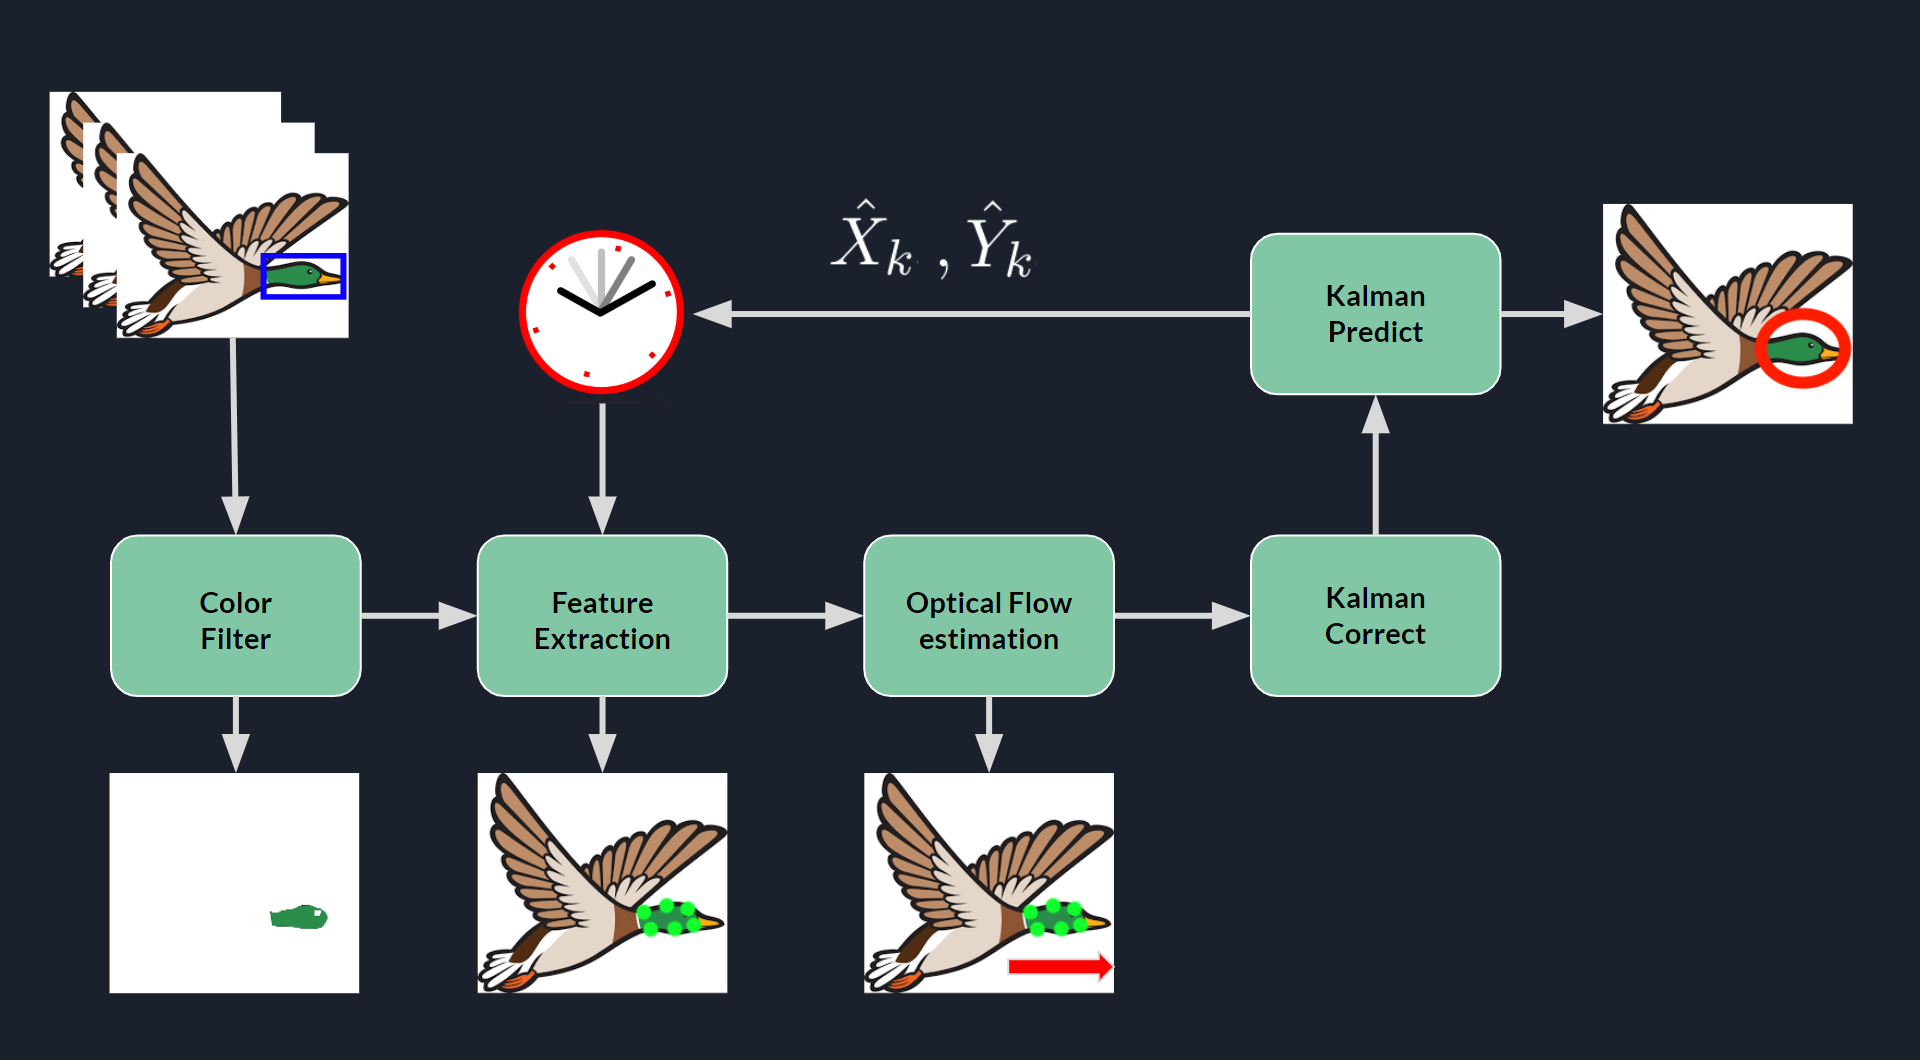
\includegraphics[width=0.5\textwidth]{Imagenes/diagram.png}
%	\caption{Diagrama en bloques del programa.}
%	\label{fig:bloques}
%\end{figure}





































\subsubsection{Escenarios de fallas}
Si bien se han minimizado las probabilidades de cometer errores de tipo I y tipo II, aún se plantean los siguientes problemas:
\begin{itemize}
%\item En caso de oclusión del objeto de interés $A$ y en la presencia de otro objeto de cualidades similares $B$ el algoritmo podrá dar un falso positivo.
%\item El cambio de trayectoria de un objeto ocluido provocará una falla en la predicción de la trayectoria, si bien a diferencia del diseño anterior, ahora no habrá problemas en retornar al objeto correcto una vez que vuelva a aparecer en pantalla.
\item El algoritmo se encuentra en su situación más frágil al haber un objecto idéntico o de gran similaridad tanto en color como en forma con el que se quiere seguir, debido a que ni el filtro de distribución de color ni el filtro de correlación lograrán distinguir entre ambos. En este caso la única distinción entre ambos será la retención de esquinas características al objeto correcto proporcionado por el algoritmo de Optical Flow. 
\item La correcta elección de parámetros de los algoritmos encargados de la fase de enmascaramiento para cada situación proporcionan una gran robustez frente a cambios en la iluminación. Sin embargo, cuanto más robusto frente a cambios en la iluminación es el algoritmo, mayor será la probabilidad de cometer errores del tipo II (seguir a un objeto incorrecto) debido a que el enmascaramiento tendrá una mayor permisividad. 
\end{itemize}



